
\chapter{\textsl{exploits}}
\label{chap:exploits}
	No presente capítulo, será feita uma breve análise sobre \textsl{exploits}.
	É importante salientar que, apenas conhecendo as técnicas usadas pelos atacantes
	torna-se possível criar defesas efetivas contra elas.
	Portanto, o estudo dessa matéria não constitui, de forma alguma, uma apologia
	ao ataque. Essa questão é muito bem abordada na parte I de \cite{Harris2008}; deixando
	claro que o conhecimento é uma arma importantíssima para aqueles que buscam
	uma melhoria na segurança do software.
	

	Como ponto de partida, será aprofundado o conceito de \textsl{exploit}. De forma
	a mostrar sua amplitude e sua intrínseca relação com as vulnerabilidades. A seguir,
	serão explicadas algumas técnicas que são representativas para uma visão ampla do assunto. 
	Na sequência, serão abordados princípios básicos de programação que visam prevenir a aplicação
	de \textsl{exploits} no software - combatem as falhas na origem e pontos de apoio usados
	pelas técnicas dos atacantes. Por fim, serão apresentadas algumas das proteções já existentes
	para barrar os ataques; em certos casos, também serão mostradas as formas de escape que
	os atacantes já desenvolveram como reação. 
	

	Como não será detalhada nenhuma técnica em particular nesse capítulo, para se obter um exemplo
	mais aprofundado de \textsl{exploit}, o \textsl{NULL pointer exploit} será o tema do capítulo seguinte.
	Assim, após um acompanhamento mais amplo do tema, será possível compreender melhor um caso específico.

	\section{Definição}
		Conforme foi tratado na Seção \ref{sec:vuln_exploit}, o \textsl{exploit} é um conjunto de passos,
		muitas vezes materializado em um programa, capaz de tirar proveito de uma vulnerabilidade.
		Para muitos, entretanto, \textsl{exploit} é sinônimo de um código em C escrito por um \textsl{hacker}
		que tem o potencial de atacar um sistema. Essa visão, todavia, é muito limitada.
		Assim como existem diversos tipos de vulnerabilidades, há muitos meios de tirar vantagem
		delas. Por vezes, basta conhecer uma série de passos, como cliques na interface
		da aplicação alvo, para para explorar uma falha.

		
		Em \cite{Hoglund2004}, encontramos a seguinte lista de possíveis consequências
		para um \textsl{exploit} bem sucedido:
		\begin{itemize}
			\item{Parada parcial ou completa do sistema(DoS);}
			\item{Exposição de dados confidenciais;}
			\item{Escalada de privilégios;}
			\item{Execução de código injetado pelo atacante;}
		\end{itemize}
		Logo, ao explorar uma vulnerabilidade, podem ser gerados impactos na integridade, na confidencialidade
		ou na disponibilidade de um sistema.


		De modo geral, o grande objetivo de um atacante é conseguir executar código arbitrário
		em seu alvo. Isso, porém, nem sempre é possível. Cada vulnerabilidade, conforme analisado
		no capítulo anterior, determina um universo de possibilidades para um \textsl{exploit} que a ataque.


		Uma interessante forma de entender os \textsl{exploits}, sob a ótica de sua operação,
		está na separação deles em \textsl{\textbf{control-data}} e \textsl{\textbf{non-control-data}}.
		Conforme \cite{Chen2005}, ataques do tipo \textsl{control-data} são aqueles que
		alteram dados de controle do programa alvo (como endereço de retorno da função ou ponteiros)
		para executar código injetado ou desviar para outras bibliotecas. Os do tipo
		\textsl{non-control-data}, em contraponto, são aqueles que não alteram nenhum
		dado de controle do programa e não desviam seu fluxo de execução, mas conseguem
		alguma vantagem para o atacante - como autenticação ilegítima, elevação de privilégio, 
		leitura de dados confidenciais, etc. Ao apresentar os tipos de \textsl{exploits},
		será feito uso desse critério de classificação. Normalmente, os ataques que alteram
		estruturas de controle são aqueles que possibilitam execução arbitrária de código, enquanto
		os demais usam o próprio código da aplicação, explorando alguma falha de lógica ou de
		verificação.
		

	\section{Tipos}
		Nessa Seção, será feita uma breve explicação sobre alguns tipos de \textsl{exploits}
		existentes. Isso para que o leitor possa ter uma noção geral sobre as técnicas usadas
		pelos atacantes para explorar as vulnerabilidades no software.
		Não é, de forma alguma, uma lista exaustiva, mas contém muitos exemplos significativos.
		
		
		Abaixo, lista dos tipos abordados:
		\begin{itemize}
		 	\item{\textsl{Buffer overflow};}
			\item{\textsl{Heap overflow};}
			\item{Injeção de SQL;}
			\item{XSS(\textsl{Cross Site Scripting});}
		\end{itemize}

		\subsection{\textsl{Buffer Overflow}}
		\label{subsec:buffer_overflow}
			Um dos tipos mais bem conhecidos e um dos mais explorados. Tem um impacto
			enorme pois possibilita ao atacante a execução de código arbitrário no sistema atacado.
			O famoso artigo \textsl{Smashing the Stack for Fun and Profit} de 1996, por Aleph One,
			foi o primeiro a tratar em detalhes dessa técnica. Mas conforme, \cite{Anley2007},
			essa estratégia já vinha sendo aplicada com sucesso por mais de 20 anos antes da publicação
			do artigo de Aleph One.


			Ocorre quando a aplicação guarda dados a serem lidos dos usuário(ou de qualquer
			fonte externa) em um \textsl{buffer} alocado na pilha sem verificar
			se o que foi fornecido está dentro do limite aceitável(tamanho do \textsl{buffer}.
			Isso acaba resultando na grave falha que será apresentada abaixo.
			
			Conforme explicado na Seção \ref{sec:gerencia_memoria}, no \textsl{stack frame}
			existem valores que controlam o fluxo de execução de uma aplicação.
			Dentre eles, está o valor de retorno de uma rotina. Qualquer chamada de função
			coloca na pilha o endereço para o qual ela deve retornar após seu fim. Se esse
			valor for alterado, é possível mudar o fluxo da aplicação - fazendo
			com que ele seja desviado para outro ponto qualquer.
			

			Essa técnica tira proveito desse fato. Caso a aplicação possua alguma
			falha que permita que o usuário forneça dados maiores que o espaço
			alocado na pilha para armazená-los, o excedente acaba sobrescrevendo o
			endereço de retorno da função.
	

			É o exemplo claro de ataque \textsl{control-data}. A mudança em um dado
			de controle do \textsl{stack frame} permite a colocação de um endereço
			forjado pelo atacante para mudar o fluxo de execução do programa atacado.
			
			
			Na versão "clássica desse \textsl{exploit}, o atacante fornece
			código executável, \textsl{shellcode}, que vai além do \textsl{buffer} criado para
			armazená-lo. No final dos dados enviados, também é inserido o endereço de início
			do \textsl{buffer}, que agora contém o código do atacante, para substituir no
			\textsl{stack frame} o valor de retorno da função. Assim, no retorno o fluxo
			é desviado para o \textsl{buffer} com o \textsl{shellcode}. A figura 
			\ref{fig:pilha_buffer_overflow} mostra uma visão simplificada da pilha
			antes e depois do ataque. 

			\begin{figure}
				\begin{center}
					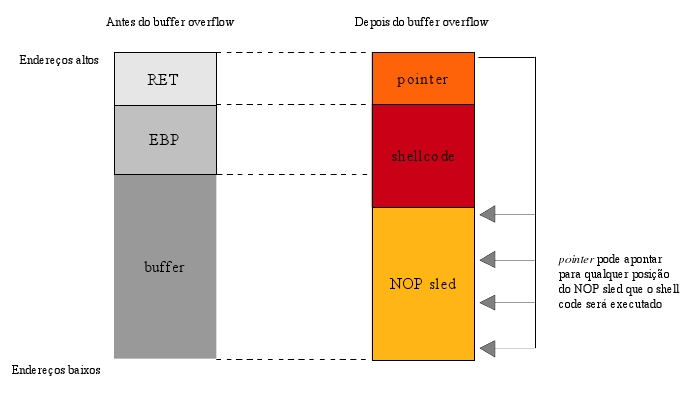
\includegraphics[width=0.90\textwidth]{pilha_buffer_overflow.jpg}
					\caption{Esquema da pilha no \textsl{buffer overflow}. Fonte: \cite{Martins2009}.}
					\label{fig:pilha_buffer_overflow}
				\end{center}
			\end{figure}

		\subsection{\textsl{Heap Overflow}}
			Semelhante ao \textsl{buffer overflow} quanto à falha que o provoca.
			Diferencia-se, entretanto, pelo fato do \textsl{buffer} a sofrer o \textsl{overflow}
			estar no heap e não na pilha. Pode ser de muito mais complexa execução que
			muitos outras técnicas - isso porque, conforme veremos, não possui o caráter
			mais genérico que seu equivalente para a pilha.
			
			
			Está diretamente relacionado à implementação feita para manejar o heap no sistema
			afetado. Isso geralmente é atribuição da biblioteca C. Logo, além da vulnerabilidade
			de \textsl{overflow}, deve estar presente uma versão de biblioteca C que faça alguma
			gerência incorreta do heap para que um ataque desse tipo seja possível.

			
			Assim, um \textsl{exploit} de \textsl{heap overflow} é totalmente focado
			em uma determinada versão de biblioteca C de um sistema, pois normalmente as aplicações
			não fazem sua própria gerência do heap. Na Seção \ref{sec:funcionamento_heap}, há
			uma explicação do funcionamento do heap que auxilia na compreensão desse tipo de ataque.
			

			Para ilustrarmos melhor esse tema, iremos focar em um sistema específico
			para mostrar a sistemática e a potencialidade de um \textsl{heap overflow}.
			Será a implementação de gerência do heap do Linux originalmente escrito por Doug Lee.
			A tarefa de controle da memória dinâmica é extremamente complexa e desafiadora, pois
			está condicionada a otimização temporal e espacial. Como muitas aplicações fazem
			uso intensivo de chamadas a malloc, free e mmap - todas para controle do heap - é preciso 
			um enorme cuidado para que os recursos de CPU e memória sejam bem utilizados de forma
			a não prejudicar o desempenho da aplicação e do sistema como um todo.


			Para manter controle do heap, nos blocos alocados e fornecidos às aplicações,
			são também postos dados de manutenção. São meta informações que visam auxiliar
			na administração dos blocos de memória. Assim, por exemplo, ao alocarmos uma porção
			de memória utilizando malloc, escondido no bloco, teremos dados que a biblioteca
			mantém.	Para a referida versão da biblioteca C do Linux, havia uma falha na qual, 
			uma vez que os metadados dos blocos fossem alterados (via \textsl{overflow}) de uma
			determinada forma, o atacante poderia conseguir uma escrita arbitrária e um endereço arbitrário.
			Conforme já abordado anteriormente, uma falha dessa magnitude implica a possibilidade
			de alteração do fluxo da aplicação caso seja sobrescrita alguma estrutura de dados de controle.
			Uma alternativa seria um ponteiro para um função - pois uma vez sobrescrito, bastaria
			que ele passasse a apontar para o código injetado pelo atacante.


			Como a intenção desse capítulo é fornecer uma visão geral, não será detalhada
			a construção do ataque. Apenas serão esboçados os passos que são seguidos pelo atacante
			para desenvolver o \textsl{exploit}.
			
			Em, \cite{Anley2007}, 
				
		
		\subsection{Injeção de SQL}
			Diferentemente dos \textsl{exploits} anteriores, não se trata de um erro de corrupção
			de memória. Serve como boa forma de contraponto para mostrar que um sistema
			pode ter sua confidencialidade e integridade afetados de outra forma.
			Ocorre na camada de banco de dados de uma aplicação em virtude de uma filtragem inadequada
			dos dados usados para gerar \textsl{queries} SQL.			

			
			Ainda que seja uma classe muito diferente, quando comparado aos 2 tipos 
			descritos anteriormente, cabe destacar que seria identificado como 
			\textsl{non-control-data}. Não é necessária nenhuma alteração no fluxo do programa
			explorado.

			
			Sua potencialidade é enorme. Como implica a possibilidade do atacante
			injetar \textsl{queries} no banco de dados do sistema alvo, significa
			dizer que ele terá todos os privilégios de acesso que a aplicação possuir.
			Pode ser possível expor informações sigilosas, alterá-las ou mesmo destruir
			toda a base de dados.


			Ataques de injeção de SQL 

		\subsection{\textsl{XSS}}
			dd

	\section{Prevenção de ataques}
		Para prevenir as indesejáveis consequências dos \textsl{exploits} apresentados
		anteriormente, mas não se restringindo a eles, serão discutidos princípios básicos
		para o desenvolvimento do software. São meios de trazer maiores garantias contra os ataques
		na origem. Será demonstrado que a validação dos dados usados pelas aplicações, bem como
		o uso de ferramentas de análise de código e de testes são exigências que não podem
		ser desconsideradas. 

		
		\subsection{Validação de dados de entrada}
			Um dos pontos primordiais para a defesa contra os ataques é a validação dos dados de entrada.
			Sendo esse procedimento capaz de deter uma série de ameaças. Uma aplicação que não verifique
			devidamente os dados que lhe são fornecidos é séria candidata a ser explorada. Não é possível
			confiar em nada que advém de qualquer ponto externo ao sistema. Conforme visto anteriormente,
			ataques como o de \textsl{buffer overflow} ou de \textsl{heap overflow} estão diretamente
			ligados a uma validação incorreta(ou mesmo ausente) de dados de entrada. O mesmo ocorrendo
			para injeção de SQL ou XSS.


			Para que essa prática seja bem aplicada, é essencial que sejam levantados todos os vetores
			de entrada de uma aplicação. Por vezes, alguns deles podem ser esquecidos. No ambiente UNIX,
			por exemplo, variáveis de ambiente também devem ser consideradas dados de entrada. Entretanto,
			nem sempre são devidamente validadas. Nesse aspecto, toda uma preocupação com a entrada
			do sistema pode ser perdida se restar apenas um ponto não verificado. Por isso a exigência
			de uma avaliação dos pontos que devem ser protegidos.


			Para ilustrar ainda melhor, podemos tomar como exemplo um sistema que faça uso de 
			DNS reverso\footnote{Processo de descoberta do nome associado a um dado IP.}. Se, para um
			dado IP, não for validado o nome retornado pelo DNS reverso, um atacante pode, uma vez que
			tenha comprometido parte da rede, forçar a aplicação a utilizar dados impróprios.
			Se a aplicação do exemplo usar diretamente o resultado, ela corre sérios riscos de sofrer
			algum tipo de exploração - como um \textsl{buffer overflow}.


			É, fundamental, portanto, que os pontos de entrada sejam identificados e sejam
			definidas formas de validação. Em \cite{Secure2006}, anexo B, há detalhes sobre
			esse tópico - definindo diretivas para a validação.
			
		\subsection{Ferramentas de análise estática e auditoria de código}
			Uma das melhores formas de prevenção a ataques é auditar o código. 
			A busca por falhas não precisa ser um procedimento manual; há uma série de ferramentas,
			algumas delas sofisticadas e focadas nessa tarefa, que podem facilitar muito a vida
			dos desenvolvedores.
			Nessa Seção, iremos abordar essa estratégia na busca por problemas 
			que possam ser eliminados já na fase de desenvolvimento - procurando
			deixar o mínimo possível de brechas para os atacantes.
			
			
			Conforme \cite{Ari2008}, a auditoria de código cai na categoria de teste
			estrutural caixa-branca. Isso porque parte do código fonte para desempenhar sua tarefa.
			O mesmo autor também destaca que esse processo,
			assim como os testes fuzzing(vide capítulo \ref{chap:fuzzing}), não é
			\textsl{capaz de comprovadamente encontrar todos os \textsl{bugs} ou erros possíveis}. 
			Ainda assim, ele recomenda fortemente seu uso em complementação a outras técnicas
			de testes(como o fuzzing ou outros tipos de teste caixa-preta).


			Muito embora o uso de ferramentas estáticas não possa substituir um auditor experiente,
			conforme ressalta \cite{Anley2007}, elas podem servir de base para a tarefa.
			Essa afirmação desse autor 

		\subsection{Testes}
		
	
	\section{Proteções e contra-proteções}
	\label{sec:exploit_protection}
		Existem diversas proteções para impedir um \textsl{exploit}.
		São recursos dos compiladores, das bibliotecas, do hardware e dos sistemas operacionais
		que servem de contra ponto às mais variadas técnicas que os atacantes já criaram.
		Seu principal objetivo é resguardar os sistemas mesmo que os desenvolvedores
		não tenham seguido as recomendações de segurança. De forma que, mesmo na presença de uma
		vulnerabilidade, um ataque não seja possível ou seus efeitos sejam minimizados ao máximo.
		
		
		Conforme é possível encontrar em \cite{Anley2007}, destacamos os seguintes mecanismos
		de proteção:
		\begin{enumerate}
			\item{Pilha não executável;}
			\item{W \^\ X(permissão de escrita ou de execução - nunca ambas);}
			\item{Canário para pilha;}
			\item{Reordenamento das variáveis na pilha;}
			\item{ASLR - Randomização do espaço de endereços;}
		\end{enumerate}

		
		A seguir, cada uma será explicada em seus aspectos fundamentais.
		\subsection{Pilha não executável}
			A primeira, pilha não executável, é uma reação natural a um dos ataques mais comuns:
			o \textsl{buffer overflow}. Há registros de propostas de pilha não executável desde 1996 -
			conforme \cite{Anley2007}(pg. 376). O \textsl{exploit} clássico sendo baseado na cópia
			de \textsl{shell code} para o buffer e posterior execução dele ficaria impraticável.
			Mas não demorou muito para os atacantes reagirem. Surgiram novas técnicas que funcionam
			mesmo quando não é possível executar o código injetado na pilha.
			Sua estratégia básica era: a partir do controle do \textsl{stack frame}, criar uma chamada
			válida para biblioteca C ou chamadas de sistema. Inicialmente, ela foi denominada \textbf{return-into-libc}.
			
			
			Essa nova técnica de \textsl{exploit} abriria caminho para uma série de outras.
		

		\subsection{W\^\ X}
			Impedir que memória com proteção de escrita seja executável e, bloquear a escrita
			para aquela que é executável é uma das melhores formas de proteção.
			Ataca justamente um princípio fundamental da maioria das técnicas de ataque: injetar código
			(escrever) e executá-lo.	
			

			Embora essa técnica seja hoje em dia conhecida pelo batismo de Theo Raadt, desenvolvedor
			e líder do projeto do OpenBSD, ela tem sua origem na década de 1970. Em \cite{Anley2007},
			é mencionado que o sistema Multics teria sido um dos pioneiros a contar com esse tipo de
			proteção. Para facilitar essa estratégia de defesa na arquitetura x86, em 2003, a AMD
			criaria o \textbf{NX(Non-eXecutable)}. Um suporte no hardware que identificasse uma página de
			memória que não pudesse ser executada. O equivalente da Intel seria o \textsl{ED(Execute Disable)}.


			Mesmo sendo uma excelente forma de impedir ataques, isolada, essa defesa não é capaz
			suficiente. Algumas técnicas derivadas de \textsl{return-into-libc} são imunes.


		\subsection{Canário para a pilha}
			Outra forma de proteção para a pilha é colocação de um canário.
			Trata-se de um valor(normalmente de 32 bits) que é posto no \textsl{stack frame}
			para identificar se houve um \textsl{overflow} na pilha.
			A figura \ref{fig:canario} ilustra essa proteção. O canário é posto de forma
			a proteger o endereço de retorno. Ao término da chamada da função, ele é verificado
			e, caso não seja o valor esperado, a aplicação é terminada.


			Sua primeira implementação foi o  \textsl{StackGuard} em 1998, vindo a fazer
			parte do compilador GCC(GNU Compiler Collection) - posteriormente sendo
			substituído pelo SSP(\textsl{Stack-Smashing Protector}) \cite{Martins2009}.
			O SSP além de implementar proteção por canário, também atua reordenando
			as variáveis da pilha para aumentar a segurança - conforme explicado 
			na Seção \ref{subsec:reordenamento_pilha}.

			
			Atualmente é uma proteção padrão em quase todos os sistemais operacionais e certamente
			contribui muito para frear \textsl{exploits} de \textsl{buffer overflow}. Sua
			proteção é ainda maior quando combinada com o reordenamento da pilha.
			

			\begin{figure}
				\begin{center}
					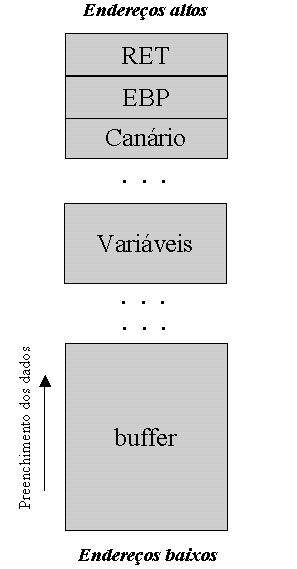
\includegraphics[width=0.30\textwidth]{canario.jpg}
					\caption{\textsl{Stack frame} protegido por canário. Fonte: \cite{Furlan2005}.}
					\label{fig:canario}
				\end{center}
			\end{figure}

		\subsection{Reordenamento de variáveis na pilha}
		\label{subsec:reordenamento_pilha}
			É aplicada pelo SSP e complementa a proteção oferecida pelo canário.
			É uma barreira extra para que um \textsl{overflow} nos \textsl{buffers} - que só
			é detectado após o término da função - não seja usado para afetar outras variáveis.


			Seu objetivo é, conforme \cite{Martins2009}:
			"isolar os arrays que podem vir a vazar dados, para que seu estouro não
			afete as outras variáveis locais da função. Isso garante a integridade das variáveis
            automáticas no decorrer da função, e evita o seu possível uso para a injeção de \textsl{shellcode}".

			
			É baseada em um modelo ideal de pilha no qual as variáveis locais que não
			são \textsl{buffers} são melhor protegidas contra possíveis \textsl{overflows}.
			O modelo é melhor compreendido através da visualização da figura \ref{fig:pilha_ideal_ssp}.

			\begin{figure}
				\begin{center}
					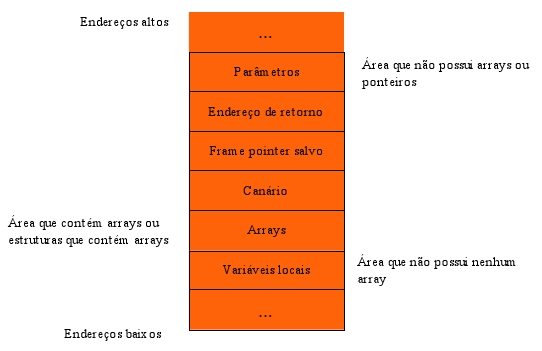
\includegraphics[width=0.80\textwidth]{pilha_ideal_ssp.jpg}
					\caption{Modelo de pilha ideal para o SSP. Fonte: \cite{Martins2009}.}
					\label{fig:pilha_ideal_ssp}
				\end{center}
			\end{figure}


		\subsection{ASLR}
			O \textsl{\textbf{Address Space Layout Randomization}} implementa uma randomização
			dos endereços de forma a dificultar enormemente a vida dos atacantes.
			Bibliotecas e rotinas passam a ter endereços aleatórios e os saltos necessários
			para esses endereços ficam muito mais complexos de serem realizados.

			
			Conforme explicado anteriormente, vários \textsl{exploits} dependem de um conhecimento
			prévio dos endereços. Portanto, essa aleatoriedade é muito interessante como
			forma de proteção genérica. Sua fraqueza, porém, conforme \cite{Anley2007}, está no fato
			de bastar algum endereço fixo para que ela não tenha efeito algum. Mas nem sempre é necessário
			que haja algo fixo; há uma técnica chamada \textsl{\textbf{heap spraying}} que é capaz
			de driblar o ASLR. Ela injeta várias porções de código executável na aplicação alvo
			para que, mesmo desconhecendo um endereço preciso, a chance de que ele seja encontrado
			venha a ser muito maior.

			
			Há mais detalhes sobre \textsl{\textbf{heap spraying}} em \cite{Nozzle}. No referido trabalho,
			inclusive, é sugerido um verificador de \textsl{heap} que procura impedir que esse tipo
			de ataque sej. No referido trabalho,
			inclusive, é sugerido um verificador de \textsl{heap} que procura impedir que esse tipo
			de ataque seja aplicado.
			
			
			

		

		
			
	
